\documentclass{article}
\usepackage{pgfplots, tikz}
\usepackage{caption}
\pgfplotsset{compat=1.18}
\usetikzlibrary{arrows.meta}
\begin{document}
\begin{center}
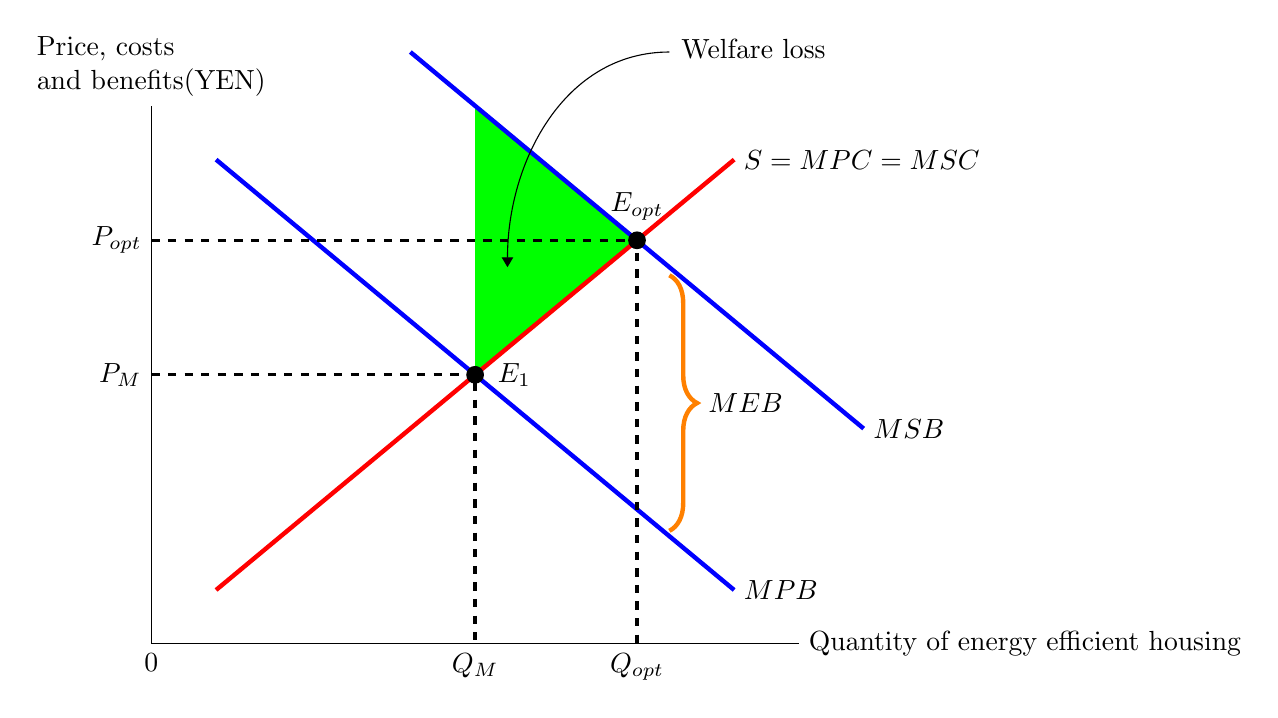
\begin{tikzpicture}
\begin{axis}[
scale = 1.2,
xmin = 0, xmax = 10,
ymin = 0, ymax = 10,
axis lines* = left,
xtick = {0}, ytick = \empty,
clip = false,
xlabel={Quantity of energy efficient housing}, x label style={at=(current axis.right of origin), anchor=west},
ylabel={Price, costs\\and benefits(YEN)}, y label style={align=left, at=(current axis.above origin), anchor=south, rotate=-90},
]

% Colouring areas
\fill[green, opacity = 15] (5, 5) -- (5, 10) -- (7.5,7.5);
% MPB line
\addplot[color = blue, ultra thick] coordinates {(1, 9) (9, 1)};
% MSB line
\addplot[color = blue, ultra thick] coordinates {(4, 11) (11, 4)};
% S line
\addplot[color = red, ultra thick] coordinates {(1, 1) (9, 9)};
% MEB curve
\draw[color=orange, ultra thick, decorate, decoration={brace, amplitude=10pt}]
    (8,6.85) -- (8,2.1) node[midway, right, xshift=10pt, color=black] {$MEB$};
% E_1 Dashed lines
\addplot[color = black, dashed, very thick] coordinates {(0, 5) (5, 5)
    (5, 0)};
%shaded region
\node [above] at (9.3, 10.7) {Welfare loss};
\draw[-Triangle] (8, 11) to [out = 180, in = 90] (5.5, 7);
% E_opt Dashed lines
\addplot[color = black, dashed, very thick] coordinates {(0, 7.5) (7.5, 7.5)
    (7.5, 0)};
% E_1 Coordinate point
\addplot[color = black, mark = *, only marks, mark size = 3pt]
    coordinates {(5, 5)};
% E_opt Coordinate point
\addplot[color = black, mark = *, only marks, mark size = 3pt]
    coordinates {(7.5, 7.5)};
% Axis Labels
% Equillibrium Labels
\node [right] at (5.2, 5) {$E_1$};
\node [above] at (7.5, 7.7) {$E_{opt}$};
% Price Axis Labels
\node [left] at (0, 5) {$P_M$};
\node [left] at (0, 7.5) {$P_{opt}$};
% Quantity Axis Labels
\node [below] at (5, 0) {$Q_M$};
\node [below] at (7.5, 0) {$Q_{opt}$};
% Line Labels
\node [right] at (9, 1) {$MPB$};
\node [right] at (9, 9) {$S= MPC= MSC$};
\node [right] at (11,4) {$MSB$};
\end{axis}
\end{tikzpicture}
\captionof{figure}{\textbf{Positive consumption externality in the energy efficient housing market}}
\end{center}
\end{document}